\documentclass{article}
\usepackage[utf8]{inputenc}

%References
\usepackage{hyperref}

%Colors
\usepackage{xcolor}


%Code Markup
\usepackage[outputdir=cache]{minted}
%Syntax Highlighting Style
\definecolor{bggray}{RGB}{40,40,40}
\newmintedfile[javacode]{java}{
	style=fruity,
	bgcolor=bggray,
	linenos,
	breaklines
}

%Page Margins and stuff
\usepackage{geometry}
 \geometry{
 a4paper,
 total={170mm,257mm},
 left=20mm,
 }

%Pictures
\usepackage{graphicx}
\graphicspath{ {./images/} }

%Move the title position
\usepackage{titling}

\setlength{\droptitle}{-8.5em} %Up, near the top but not too high

\title{Assignment 1 - Object Oriented Programming}
\author{Daniel Hannon (19484286)}
\date{October 2020}

\begin{document}
	\maketitle
	\section{Overview}
	Within this assignment we have to model a car. There's three components in particular that we look at: Car, Engine, and Wheel.\\
	For the car, I imagined it as the body of the car, holding the spedometer and keeping track of distance. As we were presented with the decision as to the location in which we store the fuel within the object of the car, I decided to store it in the Engine as it is more vital for the Engine to have direct access to the fuel than it is the car. \\ As the engine is a solid object, I felt that you didn't require to modify the basic parameters of the engine for they would not change in a solid block engine, the same applied for the wheel. At Initilaisation of Wheel, I felt it would make sense to calculate circumference as it would remain a constant for the entire lifecycle of the wheel. \\ I wrote error handling code for anything that requires there to be an object in a certain location within the parent object to prevent the program from crashing as much as possible. Additionally, there were a few logic checks within the code to prevent the presence of negative values in locations like TPL, Distance, and Fuel Level.
	\section{Code}
	\subsection{Car.java}
	\javacode{Car.java}
	\newpage
	\subsection{Engine.java}
	\javacode{Engine.java}
	\subsection{Wheel.java}
	\javacode{Wheel.java}
	\subsection{TestCar.java}
	\javacode{TestCar.java}
	\section{Output}
	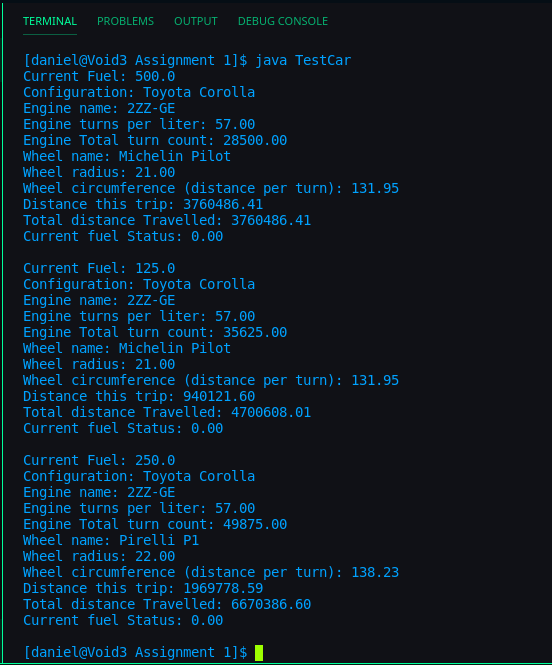
\includegraphics{testoutput.png}
\end{document}